% ==========================================
% CHAPTER 4: TRAINING & SOFTWARE
% ==========================================
\chapter{Training Design and Software Implementation}
\label{chap:implementation}

This chapter details how the architectural requirements specified in Chapter 3 are realized through training strategies and software implementation. It first presents the training design, including the metric learning objective and the evaluation framework used to validate strict generalization. Subsequently, it describes the implementation details of key system components.

\section{Model Training Strategy}

\subsubsection*{Per-Exercise Modeling Strategy}
A foundational design choice in the KinetoCheck framework is the use of independent, exercise-specific models. Rather than training a single monolithic network to evaluate all possible movements, the pipeline trains a dedicated Siamese ST-GAT model for each of the ten exercises in the UI-PRMD dataset. This one-to-one mapping is biomechanically necessary: the optimal spatial attention weights and temporal dynamics required to evaluate a deep squat are fundamentally different from those required to evaluate a lateral lunge. By isolating the training data per exercise, each model creates a highly specialized latent space focused exclusively on the nuanced degradation patterns of that specific movement, thereby preventing cross-exercise feature interference.

The training implementation is organized around a reusable trainer and three thin entry scripts. The baseline script uses a fixed XYZ-based feature pipeline (only coordinates in the 3D cartesian space), the factory-based script allows feature extraction strategies to be selected, and the phase-aware script enables auxiliary correction outputs and Range-Of-Motion (ROM) regularization.

\begin{figure}[htbp]
    \centering
    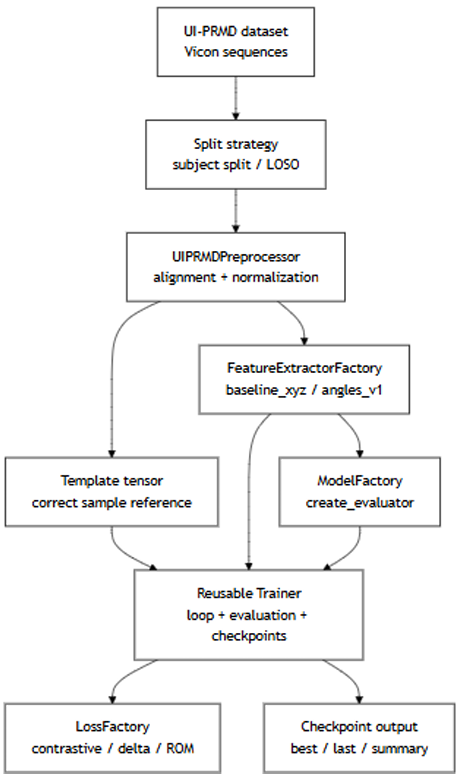
\includegraphics[width=0.9\textwidth]{figures/modular_training_architecture.png}
    \caption{The modular training architecture, highlighting the integration of the reusable trainer with feature and loss factories.}
    \label{fig:modular-training}
\end{figure}

\subsection{Spatio-Temporal Graph Attention Network Architecture}
The core processing engine of the KinetoCheck framework is the Spatio-Temporal Graph Attention Network (ST-GAT). Unlike traditional Convolutional Neural Networks (CNNs) that process dense pixel grids, or standard Recurrent Neural Networks (RNNs) that process flattened coordinate arrays, the ST-GAT preserves the explicit geometric and anatomical structure of the human body.

Building upon the theoretical graph representation established in Section 2.1.2, KinetoCheck implements the spatio-temporal graph $G$ utilizing the 17-joint MediaPipe topology. Rather than passing raw coordinates, each node $V$ is populated with the comprehensive 12-channel kinematic feature vector detailed in Section 4.2.2. The edges $E$ are strictly defined by the natural anatomical connections of the human skeleton, forming the spatial adjacency matrix used during the forward pass.

\subsubsection*{Spatial Graph Attention}
In the spatial domain, the network must understand how the movement of one joint affects its neighbors (e.g., how a collapsed knee affects the hip). Graph Attention Layers (GAT) are utilized to compute dynamic edge weights. During the forward pass, the model calculates an attention coefficient $\alpha_{i,j}$ for every pair of connected joints $i$ and $j$. This coefficient represents the biomechanical importance of joint $j$'s features to joint $i$'s current state.

This attention mechanism is the foundation of the platform’s Explainable AI (XAI) capabilities. Rather than remaining a "black box," the pooled spatial attention weights are explicitly extracted during inference and persisted into the \texttt{JointInsight} database table (as discussed in Section 4.4.2). These weights determine the Importance and Problem Score metrics, allowing the frontend to highlight specific failing joints on the user’s dashboard.

\subsubsection*{Temporal Pyramids}
Human movement occurs across multiple temporal scales simultaneously; a localized tremor might last only a few frames, while the overall repetition spans the entire sequence. To capture this without the gradient instability often associated with LSTMs, the ST-GAT implements 1D Temporal Convolutional Pyramids.

After the spatial attention layer processes the frame-wise geometry, the temporal module applies 1D dilated convolutions along the time dimension. By using parallel convolutional branches with varying receptive fields (e.g., kernel sizes of 3, 5, and 7), the network simultaneously captures high-frequency immediate anomalies (like sudden instability) and low-frequency long-term trends (like the overall speed of the repetition).

The outputs of the spatial and temporal layers are subsequently pooled into a final 128-dimensional latent embedding vector, which acts as the condensed representation of the entire exercise execution.

\subsection{Mathematical Formulation of the Contrastive Objective}
The baseline and factory-based variants optimize a contrastive loss over template and user embeddings. Rather than predicting a discrete class label, the Siamese architecture maps input sequences into a 128-dimensional latent space where the Euclidean distance between embeddings represents the biomechanical similarity of the executions.

Let $f_{\theta}(\cdot)$ denote the ST-GAT encoder parameterized by weights $\theta$. Given a template sequence $x_t$ and a user sequence $x_u$, the network generates $L_2$-normalized embeddings $z_t = f_{\theta}(x_t)$ and $z_u = f_{\theta}(x_u)$. A ground-truth label $y \in \{0, 1\}$ is provided, where $y = 1$ indicates that the user sequence is a correct execution (a positive pair), and $y = 0$ indicates an incorrect execution (a negative pair).

The optimization objective minimizes the contrastive loss function $\mathcal{L}$, defined as:
\begin{equation}
\mathcal{L}(z_t, z_u, y) = y \cdot ||z_t - z_u||_2^2 + (1 - y) \cdot \max(0, m - ||z_t - z_u||_2)^2
\end{equation}

Where:
\begin{itemize}
    \item $||z_t - z_u||_2$ is the Euclidean distance between the template and user embeddings.
    \item $m$ is the margin hyperparameter (set to 1.0 in this implementation).
\end{itemize}

During the forward pass, if the pair represents a correct execution ($y = 1$), the second term zeros out, and the network penalizes the squared distance, forcing the embeddings closer together. Conversely, if the pair is incorrect ($y = 0$), the network ignores the first term and applies a hinge loss. This hinge loss mechanism, mathematically expressed as $\max(0, m - D)$ where $D$ is the distance between embeddings, acts as a hard threshold. The margin $m$ dictates that negative pairs are only penalized if their distance is less than 1.0. Once the embeddings are pushed sufficiently far apart (i.e., $D \geq m$), the hinge loss evaluates to exactly zero, preventing the network from aggressively separating already distinct representations and thereby stabilizing the gradient updates.
This produces a continuous similarity score that is later compared against a validation-derived threshold to produce the final binary classification.

\subsubsection*{Implementation of the Contrastive Loss}
To bridge the theoretical formulation and the software architecture, the contrastive loss is implemented as a custom PyTorch module. The exact implementation used in the training pipeline is shown in Listing 4.1.

\begin{lstlisting}[language=Python, caption=PyTorch implementation of the Contrastive Loss module., label=lst:contrastive-loss, frame=single, numbers=left]
import torch
import torch.nn as nn

class ContrastiveLoss(nn.Module):
    def __init__(self, margin: float = 1.0):
        super().__init__()
        self.margin = margin

    def forward(self, emb_a: torch.Tensor, emb_b: torch.Tensor,
                labels: torch.Tensor) -> torch.Tensor:
        # Compute pairwise Euclidean distance
        distance = torch.norm(emb_a - emb_b, p=2, dim=1)

        # Loss for correct pairs (labels == 1.0)
        loss_correct = labels * torch.pow(distance, 2)

        # Loss for incorrect pairs (labels == 0.0)
        loss_incorrect = (1.0 - labels) * torch.pow(
            torch.clamp(self.margin - distance, min=0.0), 2
        )

        # Return mean loss over the batch
        return torch.mean(loss_correct + loss_incorrect)
\end{lstlisting}

As seen in Listing~\ref{lst:contrastive-loss}, the embeddings are processed in parallel batches. The \texttt{torch.norm} function computes the L2 distance across the embedding dimension (\texttt{dim=1}). The \texttt{torch.clamp} function elegantly applies the hinge mechanism for incorrect pairs, ensuring that gradients are only propagated if the distance is smaller than the configured margin. This modular design allows the \texttt{LossFactory} to instantiate the loss function dynamically based on the chosen training configuration.

\section{Data Processing and Normalization}

\subsection{Identity Leakage Mitigation}
To reduce identity leakage, subject-wise split strategies are used so that no subject appears in more than one split. The codebase also includes explicit Leave-One-Subject-Out (LOSO) utilities for stricter generalization evaluation. In preprocessing, pose sequences are centered and normalized consistently so that training and inference use the same representation.

\subsection{Kinematic Feature Engineering and 12-Channel Representation}
Raw spatial coordinates are often insufficient to fully capture the dynamic nature of physical rehabilitation exercises. To provide the ST-GAT model with a comprehensive understanding of movement biomechanics, the preprocessed 3D coordinates are expanded into a 12-channel feature representation prior to inference. For each joint at every time step, the following kinematic features are computed:

\begin{itemize}
    \item \textbf{Channels 1--3 (Spatial Position):} The normalized X, Y, and Z coordinates of the joint.
    \item \textbf{Channels 4--6 (Velocity):} The first-order temporal derivative of the position, representing the instantaneous speed and direction of the joint.
    \item \textbf{Channels 7--9 (Acceleration):} The second-order temporal derivative of the position, indicating changes in movement speed and highlighting jitter or instability.
    \item \textbf{Channel 10 (Joint Angle):} The angle formed between anatomically connected adjacent joints (e.g., the angle at the elbow formed by the shoulder and the wrist).
    \item \textbf{Channel 11 (Angular Velocity):} The temporal derivative of the joint angle, capturing the speed of rotation during the execution of the movement.
    \item \textbf{Channel 12 (Normalized Bone Length):} The distance between connected joints, normalized by the length of the torso (computed as the distance between the left hip and the left shoulder).
\end{itemize}

By incorporating velocity and acceleration alongside static position, the model successfully captures trajectory irregularities and unstable timing, which are primary indicators of poor execution quality. Furthermore, the inclusion of normalized bone ratios ensures that the resulting feature space remains robust against natural variations in subject height, body proportions, and camera distance.

\subsection{Phase-Aware Variant and Auxiliary Multi-Task Learning}
While the baseline ST-GAT encoder effectively classifies overall movement quality, clinical rehabilitation requires granular feedback regarding partial-range executions and localized joint errors. To address this, the phase-aware variant transforms the network into a multi-task learning architecture by appending two auxiliary prediction heads to the latent embedding: a Range of Motion (ROM) regularizer and a Frame Decoder.

\subsubsection*{Range of Motion (ROM) Regularization}
Patients often compensate for muscle weakness by terminating a movement prematurely. The ROM penalty continuously measures the maximum spatial displacement (amplitude) of the user’s joints and compares it against the expected amplitude of the expert template. If a user sequence is labeled as incorrect due to a truncated range of motion, the ROM penalty applies a secondary gradient update, explicitly teaching the spatial attention layers to penalize incomplete joint trajectories.

\subsubsection*{Frame-Level Error Decoding}
To further enhance the Explainable AI (XAI) capabilities, a Multi-Layer Perceptron (MLP) Frame Decoder is attached to the user embedding. This decoder projects the 128-dimensional latent representation into a 17-dimensional vector, attempting to explicitly predict the localized spatial error magnitude at each joint. This is optimized using a Mean Squared Error (MSE) loss against the ground-truth spatial delta ($\Delta X$) between the user and the aligned template.

\subsubsection*{Composite Loss Formulation}
The total multi-task loss $\mathcal{L}_{total}$ is calculated as a weighted sum of the primary contrastive objective and the two auxiliary penalties:

\begin{equation}
\mathcal{L}_{total} = \mathcal{L}_{contrastive} + \lambda_{rom} \cdot \mathcal{L}_{ROM} + \lambda_{delta} \cdot \mathcal{L}_{delta}
\end{equation}

Where $\lambda_{rom}$ and $\lambda_{delta}$ are the configurable hyperparameter weights assigned to the auxiliary objectives (detailed in Table~\ref{tab:T3}).

Benefits of this phase-aware multi-task design include:
\begin{itemize}
    \item \textbf{Targeted Supervision:} The auxiliary gradients force the network to learn correction-aware spatial representations, improving the accuracy of the extracted attention weights.
    \item \textbf{Reduced False Positives:} ROM regularization prevents the model from accidentally validating partial-range executions that otherwise maintain correct anatomical posture.
    \item \textbf{Rich Metadata:} The decoder outputs are persisted directly into the checkpoint, enabling the advanced joint-level feedback extraction (the \texttt{JointInsight} entity) utilized during inference.
\end{itemize}

Table~\ref{tab:T3} summarizes the key hyperparameters and training choices used for the reported experiments. For reproducibility, per-fold checkpoints are saved, and the training and validation splits used for each fold are stored.

\begin{table}[H]
\centering
\small
\begin{tabular}{|p{1.5cm}|p{3.5cm}|p{2.0cm}|p{2.0cm}|p{5.0cm}|}
\hline
\textbf{Group} & \textbf{Parameter} & \textbf{Value} & \textbf{Unit/Range} & \textbf{Comment} \\ \hline
model & \texttt{in\_channels} & 9/12 & channels & xyz(+velocity+acceleration) \\ \hline
model & \texttt{hidden\_channels} & (64, 128) & tuple & ST-GAT blocks \\ \hline
model & \texttt{embedding\_dim} & 128 & dim & Siamese projection head \\ \hline
model & \texttt{use\_phase\_decoder} & True & boolean & Enables temporal alignment module \\ \hline
optimizer & \texttt{learning\_rate} & 1e-3 & & Initial learning rate \\ \hline
optimizer & \texttt{weight\_decay} & 1e-4 & & L2 regularization penalty \\ \hline
optimizer & \texttt{margin} & 1.0 & & Contrastive loss margin \\ \hline
training & \texttt{delta\_weight} & 0.0 & & Frame-level correction loss weight \\ \hline
training & \texttt{rom\_weight} & 2.0 & & Range-of-motion loss weight \\ \hline
data & \texttt{batch\_size} & 8 & samples & Training batch size \\ \hline
data & \texttt{num\_workers} & 0 & threads & DataLoader workers \\ \hline
training & \texttt{epochs} & 30 & epochs & Maximum training epochs \\ \hline
training & \texttt{patience} & 10 & epochs & Early stopping patience \\ \hline
training & \texttt{seed} & 42 & & Random seed for reproducibility \\ \hline
training & \texttt{device} & auto & & Hardware accelerator \\ \hline
split & \texttt{split\_mode} & subject & & Determines data partitioning strategy \\ \hline
split & \texttt{train/val/test ratio} & 0.8/0.1/0.1 & ratio & Dataset split proportions \\ \hline
\end{tabular}
\caption{Model hyperparameters and training settings}
\label{tab:T3}
\end{table}

\subsection{Temporal Interpolation and Spatial Anchoring}
A fundamental challenge in automated movement assessment is temporal and spatial misalignment. A patient recovering from an injury will inherently execute a repetition at a different speed and possess different anatomical proportions compared to the healthy expert template. If the system were to compute error margins on a rigid, unaligned basis, a perfectly executed but slower movement would be severely penalized.

To resolve this and generate an intuitive visual overlay (the "ghost" skeleton), KinetoCheck implements a deterministic, dual-stage alignment module consisting of Linear Temporal Interpolation and Spatial Anchoring.
Before computing the temporal alignment, the system must deterministically select the baseline expert template ($T_t$) from the UI-PRMD dataset. To ensure the template reflects a natural, therapeutic execution speed, the pipeline filters all correct executions (label = 0) for a given exercise and selects the specific sequence possessing the median frame length. This dynamically extracted 'Golden Template' serves as the anchor for both the Siamese network comparison and the visual Ghost Skeleton overlay.
\subsubsection*{Linear Temporal Sequence Interpolation}
Given a user kinematic sequence of length $T_u$ and a template sequence of length $T_t$, the system maps the discrete time indices of the user's execution into the continuous temporal space of the template. For each user frame $i \in \{0, \dots, T_u - 1\}$, the corresponding fractional template index $t_i$ is computed via linear spacing:

\begin{equation}
t_i = i \cdot \frac{T_t - 1}{T_u - 1}
\end{equation}

Because $t_i$ is a continuous floating-point value, the exact template posture must be approximated using 1D linear interpolation. By isolating the lower bound index $idx_0 = \lfloor t_i \rfloor$ and the upper bound index $idx_1 = \min(idx_0 + 1, T_t - 1)$, the fractional remainder $\alpha = t_i - idx_0$ acts as a blending weight. The temporally aligned template frame $\hat{X}_t^{(i)}$ is thus computed as a weighted combination of two adjacent expert frames:

\begin{equation}
\hat{X}_t^{(i)} = (1 - \alpha) \cdot X_t^{(idx_0)} + \alpha \cdot X_t^{(idx_1)}
\end{equation}

This continuous temporal scaling ensures the ghost skeleton remains perfectly synchronized with the user's kinematic progression throughout the entire duration of the exercise, regardless of execution speed.

\subsubsection*{Spatial Anchoring and Proportional Scaling}
Once temporally synchronized, the template must be spatially normalized to match the user's specific body metrics and camera distance. The system calculates a global scaling factor $S$, derived from the median vertical distance between the distal anatomical points (the nose and the feet) across both sequences:

\begin{equation}
S = \max \left(0.5, \min \left(4.0, \frac{\text{median}(Height_{user})}{\text{median}(Height_{template})}\right)\right)
\end{equation}

Finally, a biomechanical fulcrum (such as the midpoint between the left and right hips, or the ankles) is selected as a translation anchor $A$. The temporally interpolated template frame $\hat{X}_t^{(i)}$ is centered around its own anchor, scaled by the factor $S$, and translated to match the user's spatial anchor coordinates in the 2D plane:

\begin{equation}
Ghost^{(i)} = (\hat{X}_t^{(i)} - A_{template}^{(i)}) \cdot S + A_{user}^{(i)}
\end{equation}

This combined spatio-temporal alignment allows the rendering engine to project a highly accurate, anatomically proportional, and time-locked corrective overlay directly onto the user's video feed.

\section{Pipeline Implementation}

\subsection{Video-Based Inference via MediaPipe}
For RGB input, the system uses MediaPipe Pose Landmarker to extract frame-wise 17-joint landmarks. The model infers 33 landmarks per frame; these are remapped to the 17-joint representation used during training via a deterministic mapping defined in the preprocessing layer.

\subsection{Feedback Visualization}
To expose model reasoning, the visualization module overlays the extracted skeleton on the input video and highlights the joints that are most relevant to the model output. This produces intuitive corrective cues for users and therapists.

At startup, the inference module caches loaded checkpoints in memory to avoid repeated disk I/O. Given a preprocessed pose sequence of shape \texttt{(1, C, 120, 17)}, the inference function: (1) builds the selected feature representation; (2) passes the tensor through the evaluator; (3) computes a similarity score; (4) compares the score against the learned threshold to produce a binary decision; and (5) returns a structured result object.

\subsubsection*{Spatio-Temporal Rendering and the Ghost Skeleton Overlay}
To maximize the clinical interpretability of the system, a “ghost skeleton” overlay was implemented. This visual artifact superimposes a semi-transparent representation of the optimal template movement directly onto the user’s video feed.

The geometric scaling and frame-synchronization of this overlay are handled by the deterministic alignment module detailed previously in 4.2.4. However, applying this math to in-the-wild videos introduces a final rendering challenge: Dynamic Camera Orientation Detection. Because home rehabilitation videos exhibit varying camera angles, hardcoding the lateral axis often leads to distorted 2D projections. The rendering engine automatically resolves this by measuring the shoulder separation across the X and Y dimensions, selecting the axis with the maximum geometric variance to correctly orient the template before applying the spatial anchoring equations.

This advanced rendering pipeline ensures that patients receive real-time, proportionally accurate visual cues, clearly illustrating the spatial delta between their current posture and the idealized target movement without suffering from temporal desynchronization.

\section{Application Integration}
The ASP.NET Core web interface orchestrates the request lifecycle: upload, validation, forwarding of the video to the Python analysis service, and response rendering.

\subsection{Web Interface and Request Orchestration}
\begin{enumerate}
    \item \textbf{Upload:} User selects a video file; the interface validates MIME type and file size.
    \item \textbf{Temporary Storage:} The video is written to a temporary directory with a UUID-based filename.
    \item \textbf{Pose Extraction:} MediaPipe is invoked; keypoints are logged.
    \item \textbf{Preprocessing:} Keypoints are normalized and resampled.
    \item \textbf{Inference:} The pre-trained model is loaded and a prediction is computed.
    \item \textbf{Visualization:} An annotated video is generated.
    \item \textbf{Report Generation:} A JSON report is written containing core artifacts.
    \item \textbf{Response:} The user is provided with the predicted label, score, report path, and video link.
\end{enumerate}

\begin{figure}[H]
    \centering
    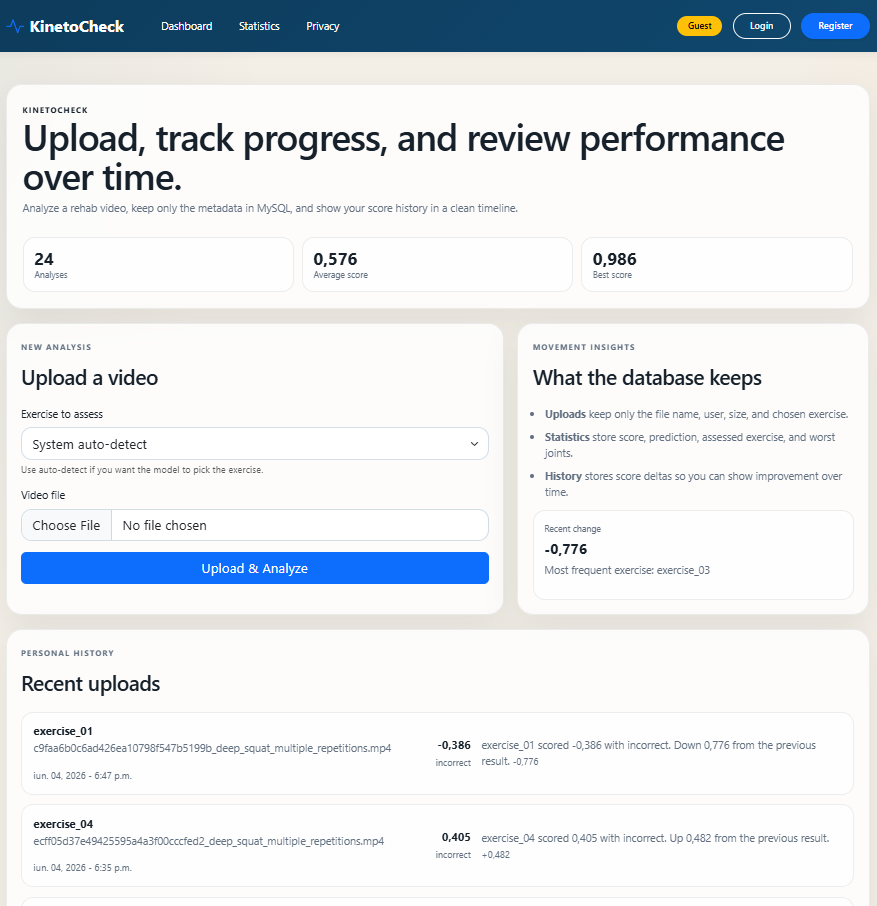
\includegraphics[width=0.9\textwidth]{figures/app_dashboard.png}
    \caption{The primary user dashboard, featuring the updated navigation bar, historical statistics, and the video upload interface.}
    \label{fig:app-dashboard}
\end{figure}

The application is designed to handle multiple concurrent requests, with asynchronous processing and caching of model checkpoints to optimize performance. Error handling is implemented at each stage to ensure that users receive informative feedback in case of issues such as invalid file formats or inference errors.

\begin{figure}[hbtp]
    \centering
    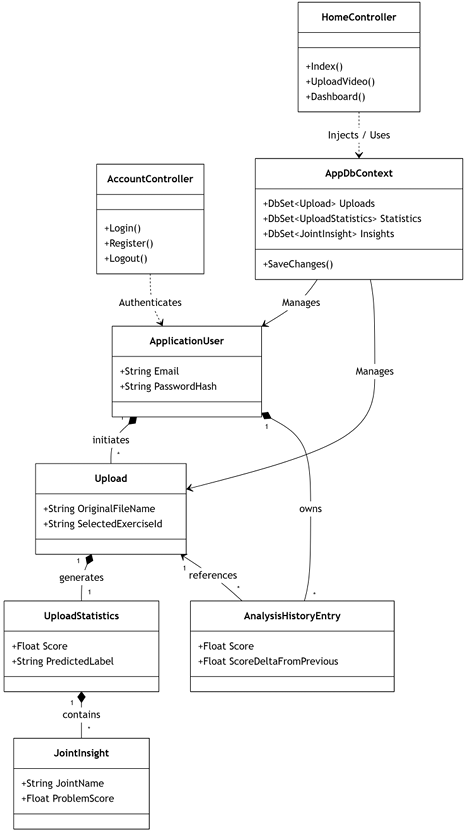
\includegraphics[width=0.8\textwidth]{figures/uml-diagram.png}
    \caption{ UML Class Diagram illustrating the core domain entities, data persistence layer, and primary web controllers.
}
    \label{fig:uml-diagram}
\end{figure}

\subsection{Data Model and Persistence (Entity Framework Core)}
Although the processing core of the KinetoCheck platform relies on deep learning models, the system operates as a comprehensive web application, requiring a robust architecture to store patient data and medical rehabilitation history. Data persistence within the .NET application is managed via Entity Framework (EF) Core. This modern Object-Relational Mapper (ORM) facilitates interaction with the relational database directly through C\# objects (via the \texttt{AppDbContext}), eliminating the need for manual SQL query construction.

To ensure strict traceability of patient progress and the decisions made by the AI model, the database was designed following normalization principles and is structured around five primary entities (illustrated in figure \ref{fig:db-diagram}):
\begin{figure}[H]
    \centering
    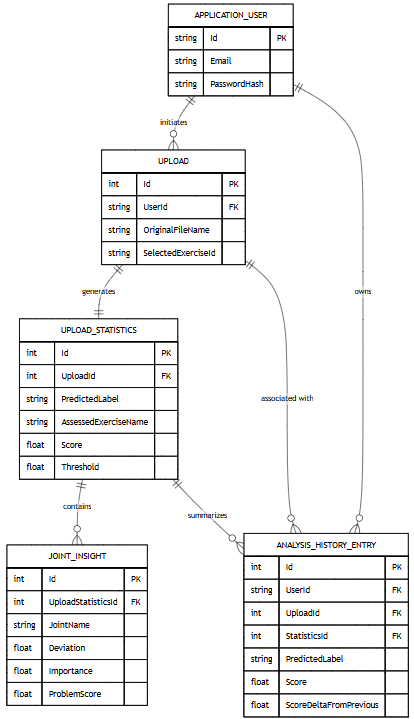
\includegraphics[width=0.7\textwidth]{figures/db-diagram.png}
    \caption{ Database Diagram illustrating the core domain entities and their relationships, as implemented via Entity Framework Core.
}
    \label{fig:db-diagram}
\end{figure}
\begin{itemize}
    \item \textbf{\texttt{ApplicationUser}:} Extends the base \texttt{IdentityUser} class from ASP.NET Core Identity. It manages profile data and account security (e.g., encrypted password hashes, session management). By utilizing the \texttt{DeleteBehavior.SetNull} constraint, the system prevents the accidental cascading deletion of aggregated medical data if a user account is ever deactivated.
    \item \textbf{\texttt{Upload}:} Represents the data entry point into the system. It stores the metadata of the original video file (\texttt{OriginalFileName}) and the identifier of the specific exercise selected by the user (\texttt{SelectedExerciseId}).
    \item \textbf{\texttt{UploadStatistics}:} Stores the raw inference results returned by the Python API in a strict one-to-one relationship with the \texttt{Upload} entity. This table captures the similarity score (\texttt{Score}), the model’s decision (\texttt{PredictedLabel}), and the automatically calibrated decision boundaries (\texttt{Threshold}, \texttt{Margin}). Isolating this data ensures rapid query execution without overloading the primary table.
    \item \textbf{\texttt{JointInsight}:} This entity is paramount for the system’s Explainable AI (XAI) capabilities. It maintains a one-to-many relationship with \texttt{UploadStatistics} and granularly stores the biomechanical errors detected at each individual joint (e.g., \texttt{Deviation}, \texttt{Importance}, \texttt{ProblemScore}). The frontend consumes this data to visually highlight problem areas (Joints of Attention) on the patient’s skeleton.
    \item \textbf{\texttt{AnalysisHistoryEntry}:} Acts as a longitudinal (time-series) evolution log. Beyond storing a textual \texttt{Summary}, it captures the \texttt{ScoreDeltaFromPrevious} metric, which automatically calculates the performance difference compared to the user’s previous execution of the same exercise. This feature is essential in a clinical context, allowing for the objective quantification of recovery progress over time.
\end{itemize}

The model utilizes strict Fluent API constraints—such as \texttt{MaxLength} and \texttt{Precision(6, 3)}—to optimize the database’s memory footprint while ensuring the strict decimal precision required by the machine learning outputs.

\subsection{Authentication and MVC Architecture}
To guarantee the confidentiality of medical data, the platform integrates a comprehensive authentication and authorization module. The entire user interaction flow is built upon the Model-View-Controller (MVC) design pattern, native to the ASP.NET Core environment.

\subsubsection*{Authentication and Access Restriction}
Access to the video analysis functionalities and medical history is strictly restricted to authenticated users. The login system, managed by the \texttt{AccountController}, employs secure Cookie Authentication to maintain active user sessions across HTTP requests. When an unauthenticated user attempts to access a protected route marked with the \texttt{[Authorize]} attribute, the security middleware automatically intercepts the request and redirects the client to the login page, thereby preventing the exposure of sensitive data.

\begin{figure}[htbp]
    \centering
    
\includegraphics[width=0.7\textwidth]{figures/app_login.png}
    \caption{The KinetoCheck authentication interface, ensuring that medical analysis history remains secure and accessible only to registered users.}
    \label{fig:app-login}
\end{figure}

\subsubsection*{The Lifecycle of an Analysis Request (MVC)}
Communication between the patient and the artificial intelligence service is elegantly orchestrated through the three components of the MVC architecture:

\begin{enumerate}
    \item \textbf{View (Graphical Interface):} The frontend is constructed using Razor Pages (HTML5 with embedded C\#). The interface includes client-side validation to ensure correct file formatting before data is transmitted to the server, preserving bandwidth and preventing unnecessary backend processing.
    \item \textbf{Controller:} The application logic is cleanly separated into dedicated controllers. While the \texttt{AccountController} handles security and the \texttt{SamplesController} manages reference data, the \texttt{HomeController} acts as the primary orchestrator for the analysis pipeline. It receives the video upload from the View, temporarily stores it, and initiates an asynchronous HTTP request to the Python analysis API (FastAPI). The asynchronous nature of this call (\texttt{async/await}) is critical, allowing the .NET server thread to remain responsive and serve other users while waiting for the neural network to finish its compute-heavy operations.
    \item \textbf{Model:} Once the JSON response is returned by the AI service, the \texttt{HomeController} deserializes the payload. The data is mapped to the previously established database entities (such as \texttt{UploadStatistics} and \texttt{JointInsight}), persisted via Entity Framework Core, and the final View is rendered to display the results and the annotated ghost skeleton to the patient, thereby completing the feedback loop.
\end{enumerate}

\subsection{Error Handling and Robustness}
The implementation follows the error handling specification from Chapter 3. Key error scenarios include: invalid video input, insufficient pose quality, checkpoint mismatch, and timeout conditions. For each scenario, the system provides user-friendly error messages and avoids producing ambiguous partial outputs.

\begin{figure}[htbp]
    \centering
    
\includegraphics[width=0.8\textwidth]{figures/app_error_handling.png}
    \caption{UI error message for missing human subjects.}
    \label{fig:app-error}
\end{figure}

\begin{figure}[htbp]
    \centering
    
\includegraphics[width=0.8\textwidth]{figures/missing_human_error_handling.png}
    \caption{UI error message for image uploads.}
    \label{fig:missing-human-error}
\end{figure}